\subsection{Dataset}

HypfuNN was developed as CAFA~\citep{CAFA} entry competing against function prediction methods by other student groups. In order to compare the fitness of the implemented prediction methods, a common
dataset for training and testing for all groups was used, as described in the implementation part. The dataset contains 2815 HPO-annotated proteins.

\subsection{Implementation}

As already described above, we predict protein annotations by homology. Proteins, that have the same function, so called homologs, tend to share a similar sequence. In order to identify proteins
with similar sequence, we are using blast and hhblits. For both, blast and hhblits, we require an minimal e-value of 1, to exclude weak similar protein sequences. Our tool supports to use
different blast e-value with the commandline option -e, as well as looking up similar proteins in other databases with the commandline options -b for blast and -l for hhblits.\newline
In order to map the annotations of the found proteins to the query sequence, our tool is looking up the annotations for each found similar sequence hit. This step is done by an identifier hpo terms mapping
file. Our method support the use of different mapping files with the commandline option -c.\newline
Since hpo is a hierarchical annotation system, each found annotation represent a tree. In order to merge these annotation trees, each node of each tree is annotated with information about the sequence
hit. Hereby our method supports the fact, that some hpoterms have more than a single parent node.\newline
\begin{figure}[!hb]
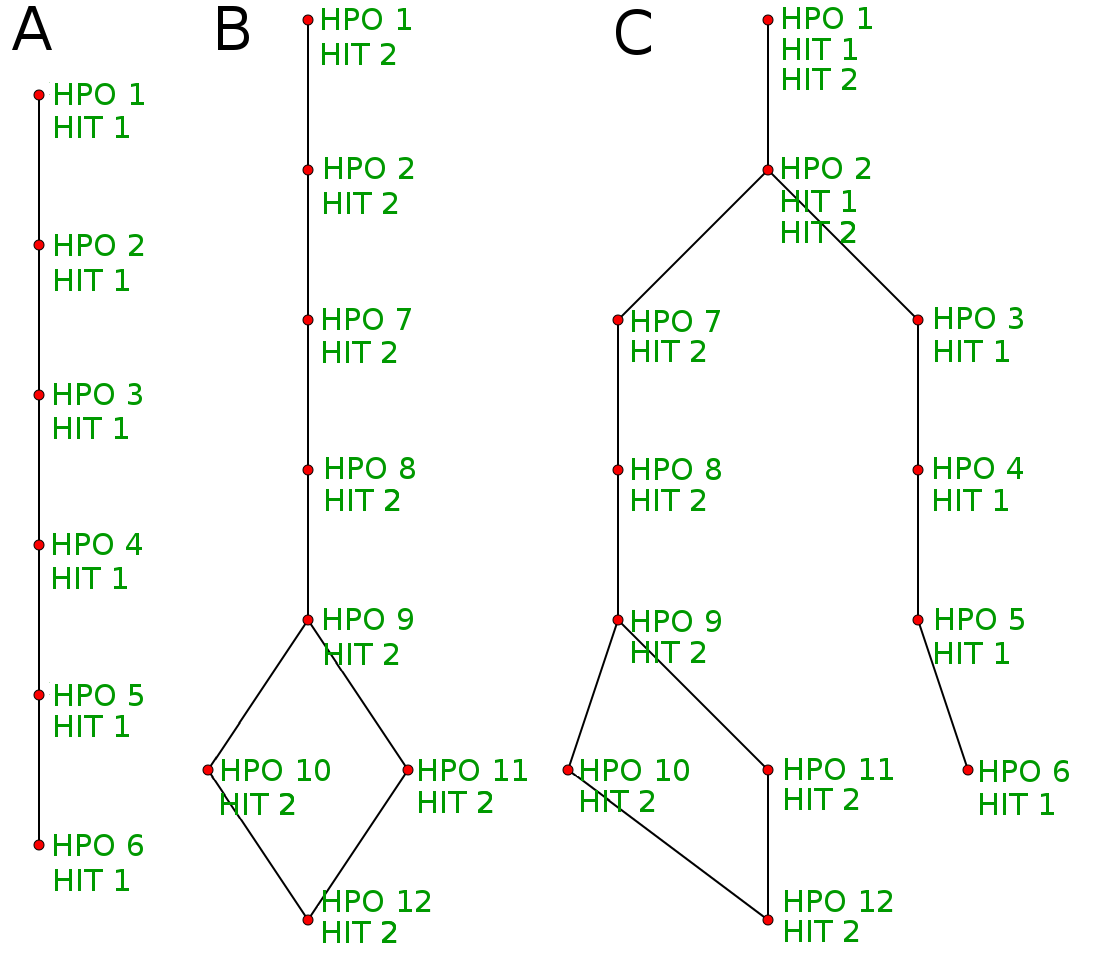
\includegraphics[width = 0.4\textwidth]{figures/merge_trees.png}
\caption{Merge trees TODO}
\label{fig:function_transfer}
\end{figure}
In order to predict whether a single annotation node can be transfered to the query sequence, we merge the found subtrees together (Figure \ref{fig:function_transfer}). By default, for the tree merging,
all subtrees are taken into account. However when calling our method with the commandline option --fast, only the annotation trees for the best 6 hits (by e-value) will be merged.\newline
Using the pyBrain\footnote{citation} toolkit, we trained a neuronal network, to find annotation nodes that may be transfered to the query sequence. For this step, the following features were taken into
account:
\begin{itemize}
\item the length of the query sequence.
\item the number of hits that have/support this annotation.
\item the longest range length of all hits having this annotation.
\item the average range length of all hits having this annotation.
\item the best e-value of all hits having this annotation.
\item the average e-value of all hits having this annotation.
\item thr product of the e-value from all hits having this annotation.
\item whether the hit with the best e-value was found by the blast or hhblits.
\item the minimal distance of the annotation to the annotation root.
\item the maximal distance of the annotation to the annotation root. (Since some root may have multiple parent nodes, this feature may differ to the above feature.)
\item the coverage of the sequence length, that have similar regions in other hits having this annotation.
\item the length of the longest hit of all hits having this annotation.
\end{itemize}
The used neuronal network has an input node for each of the above mentioned features, as well as two hidden layers. The first hidden layer contains features + 1 nodes, while the second hidden layer
contains 3 nodes. The first output node predict whether we may transfer the given annotation to the query sequence. The second output node predicts whether we may not transfer the annotation.
The difference between the two output nodes is taken as the methods confidence.
